\graphicspath{{figtema3/}}

\chapter{Medidas de tendencia central}

\section{Introducci\'on}
En el tema anterior hemos definido el concepto de frecuencia
(absoluta o relativa), en relaci\'on a una colecci\'on de datos 
estad\'isticos.

El conjunto de valores de frecuencia 
asociados a una variable estad\'istica se conoce como 
\textbf{distribuci\'on de frecuencias} de la variable.

Por ejemplo, en el tema anterior hemos utilizado las siguientes distribuciones
de frecuencias:

\vskip 0.2 cm
\begin{center}
\begin{tabular}{cc}
\begin{tabular}{|c|c|}
\hline
\textit{Nacionalidad} & Frecuencia absoluta \\ \hline
Colombia & 350 \\ \hline
Ecuador & 250 \\ \hline
Per\'u & 120 \\ \hline
Argentina & 100 \\ \hline
Ruman\'ia & 80 \\ \hline
Marruecos & 70 \\ \hline
Senegal & 30 \\ \hline
\end{tabular}
&
\begin{tabular}{|c|c|}
\hline
\textit{Edad} & Frecuencia absoluta \\ \hline
18 & 120 \\ \hline
19 & 150 \\ \hline
20 & 90 \\ \hline
21 & 70 \\ \hline
22 & 65 \\ \hline
23 & 50 \\ \hline
24 & 30 \\ \hline
25 & 20 \\ \hline
26 & 10 \\ \hline
27 & 7 \\ \hline
28 & 8 \\ \hline
29 & 2 \\ \hline
30 & 1 \\ \hline
34 & 1 \\ \hline
35 & 1 \\ \hline
40 & 1 \\ \hline
\end{tabular}
\\
Inmigraci\'on por nacionalidades & Edad estudiantes UIB 
\end{tabular}

\end{center}

En un caso la variable es \textit{Nacionalidad} (variable cualitativa)
y la distribuci\'on de frecuencias muestra el n\'umero de inmigrantes de cada
nacionalidad.
En el otro caso la variable es \textit{Edad} (variable cuantitativa) y 
la distribuci\'on de frecuencias representa el n\'umero de estudiantes de la UIB 
(de una muestra de 1000) seg\'un su edad.

En el primer caso la distribuci\'on de frecuencias consta de 7 valores. Estos valores 
describen los datos brutos relativos a 1000 personas (tabla \ref{tabla0} del tema anterior). 
Por otra parte, en el ejemplo sobre los estudiantes de la UIB, los 16 valores 
de la distribuci\'on de frecuencias resumen 626 datos brutos. Resulta evidente que
leer una tabla formada por 7 valores resulta mucho m\'as sencillo que leer una formada
por 1000 valores (del mismo modo es m\'as f\'acil leer 16 valores que 626), pero
?`es posible describir estas distribuciones de una manera a\'un m\'as resumida,
con dos o tres valores?. La respuesta a esta pregunta la damos en el presente tema.


\section{Moda, mediana y media}
En este tema veremos c\'omo describir las distribuciones de frecuencia de una variable
mediante unos pocos par\'ametros (llamados \textbf{estad\'isticos}) 
que resumen su comportamiento (o \textit{tendencia}) global. Estos estad\'isticos
reciben el nombre de estad\'isticos de tendencia central. En el siguiente tema 
es\-tu\-dia\-re\-mos otro tipo de estad\'isticos (llamados de \textit{dispersi\'on})
que completan la descripci\'on de la distribuci\'on de frecuencia.

Definimos tres estad\'isticos de tendencia central:
\begin{itemize}
\item La \textbf{moda} es el valor (o valores) con la m\'axima frecuencia.
La moda se define tanto para variables cualitativas como ordinales o 
cuantitativas.

Para el ejemplo sobre la inmigraci\'on la moda es igual a \textit{Colombia},  
pues tiene una frecuencia de $350$, mayor que la del resto de valores de 
la variable \textit{Nacionalidad}.

Para el ejemplo sobre los estudiantes de la UIB la moda es igual a $19$
pues su frecuencia es $150$, mayor que el resto de frecuencias.

Si el valor m\'aximo de la distribuci\'on se produce para dos valores distintos
de la variable  decimos que la distribuci\'on es de tipo \textbf{bimodal}.
Si se produce para un \'unico valor (como en los ejemplos comentados) se dice que
la distribuci\'on es \textbf{unimodal}.

Un ejemplo de distribuci\'on bimodal es el siguiente:

\begin{center}
Apellidos m\'as frecuentes en Illes Balears (fuente INE)
\vskip 0.2 cm
\begin{tabular}{|c|c|}
\hline
\textit{Primer apellido} & Frecuencia relativa (por 1000 habitantes) \\ \hline
GARCIA &	15,0 \\ \hline
PONS	& 15,0 \\ \hline
TORRES	& 11,9 \\ \hline
MARTINEZ	& 11,0 \\ \hline
FERRER	& 9,5 \\ \hline
FERNANDEZ	& 9,2 \\ \hline
LOPEZ	& 9,0 \\ \hline
SANCHEZ	& 8,9 \\ \hline
SERRA	& 8,7 \\ \hline
RIERA	& 8,2 \\ \hline
\end{tabular}
\end{center}

Observamos como los apellidos ``Garcia'' y ``Pons'' presentan el mismo m\'aximo de
frecuencia, por lo que la moda de la distribuci\'on es doble.

\item La \textbf{mediana} es aquel valor que, cuando consideramos todos los valores de la 
muestra ordenados, ocupa el lugar central.
Es decir, la mitad de las frecuencias est\'an por encima de la mediana y la otra mitad
por debajo. 

En la pr\'actica la mediana se calcula utilizando la siguiente propiedad:
la mediana es el menor valor de la variable cuya \textit{frecuencia acumulada} 
es mayor o igual a la mitad de la suma de todas las frecuencias. 

Recordemos que la frecuencia
acumulada se defini\'o en el tema anterior para variables que admiten una ordenaci\'on
de sus valores (variables ordinales o cuantitativas).
En este caso, la frecuencia acumulada del valor que ocupa la posici\'on $i$
es igual a la suma de su frecuencia y las de los valores anteriores: $N_i=n_1+n_2+\cdots+n_i$.

Por lo tanto la mediana es el primer valor que ocupa la posici\'on $i$ tal que $N_i \geq 0.5 \cdot N$,
o lo que es lo mismo $N_i \geq 50\% \cdot N$,
donde $N$ es la suma de todas las frecuencias. La mediana s\'olo puede definirse para variables ordinales o
cuantitativas, ya que para las variables cualitativas no tiene sentido calcular frecuencias acumuladas.

Por ejemplo, en el caso de la tabla de edades de los estudiantes de la UIB, tenemos las 
siguientes frecuencias acumuladas:

\vskip 0.2 cm
\begin{center}
\begin{tabular}{|c|c|c|}
\hline
\textit{Edad} & Frecuencia absoluta & Frecuencia acumulada \\ \hline
18 & 120 & 120\\ \hline
19 & 150 & 270\\ \hline
20 & 90 & 360\\ \hline
21 & 70 & 430\\ \hline
22 & 65 & 495\\ \hline
23 & 50 & 545\\ \hline
24 & 30 & 575\\ \hline
25 & 20 & 595\\ \hline
26 & 10 & 605\\ \hline
27 & 7 & 612\\ \hline
28 & 8 & 620\\ \hline
29 & 2 & 622\\ \hline
30 & 1 & 623\\ \hline
34 & 1 & 624\\ \hline
35 & 1 & 625\\ \hline
40 & 1 & 626\\ \hline
\end{tabular}
\end{center}

\vskip 0.2 cm
La suma de todas las frecuencias es $626$ por lo que $50\% \cdot 626=313$. Vemos que 
a partir del $3^{er}$ valor las frecuencias acumuladas son ma\-yo\-res o iguales a $313$,
por lo que la mediana es el valor que ocupa la tercera posici\'on en la tabla: mediana=$20$.
Observemos que por encima de la mediana la suma de las frecuencias (incluyendo la frecuencia
de la mediana) es $120+150+90=360$, mientras que por debajo es $90+70+65+50+30+20+10+7+8+2+1+1+1+1=356$,
es decir, aproximadamente el mismo valor.

\vskip 0.3 cm
Un concepto relacionado con el de mediana es el de \textbf{percentil}.
Si el $50\%$ de las frecuencias est\'an por encima de la mediana, 
el percentil $P$ se define de manera que el $P\%$ de las frecuencias
est\'an por encima suyo. El percentil $P$ es el primer valor que ocupa la 
posici\'on $i$ tal que $N_i \geq P\% \cdot N$.

\vskip 0.2 cm
Por ejemplo, el percentil $30$ de la tabla anterior es $19$, que ocupa la posici\'on $2$
de la tabla, ya que $30\% \cdot 626=187,8$, $N_1=120 < 187,8$, $N_2=270 > 187,8$.

\vskip 0.2 cm
El percentil $80$ es $23$, que ocupa la posici\'on $6$
de la tabla, ya que $80\% \cdot 626=500,8$, $N_5=495 < 500,8$, $N_6=545 > 500,8$.

\vskip 0.3 cm
Los percentiles $25$, $50$ y $75$ se denominan, respectivamente, primer, segundo y
tercer \textbf{cuartiles}. Por ejemplo, el tercer cuartil de la tabla anterior es
$22$, que ocupa la posici\'on $5$ de la tabla, 
ya que $75\% \cdot 626=469.5$, $N_4=430 < 469.5$, $N_5=495 > 469.5$.


\item La \textbf{media} (o media aritm\'etica, denotada $\bar{x}$)
es el valor medio de los valores de la variable, calculado 
en funci\'on de las frecuencias de la distribuci\'on seg\'un la siguiente f\'ormula:
\[
\bar{x}=\frac{n_1 \cdot x_1 + n_2 \cdot x_2 + \cdots + n_k \cdot x_k}{N}
\]
\noindent
donde $x_1, x_2, \cdots, x_k$ son los distintos valores de la variable,
$n_1, n_2, \cdots, n_k$ sus frecuencias, $k$ el n\'umero de valores distintos
que toma la variable y $N=n_1+n_2+\cdots+n_k$.

La media s\'olo puede calcularse para variables cuantitativas. Para el ejemplo
sobre los estudiantes de la UIB tenemos que:
\[
\bar{x}=\frac{120 \cdot 18 + 150 \cdot 19 + 90 \cdot 20 + \cdots + 1 \cdot 34 + 1 \cdot 35 + 1 \cdot 40}
{120+150+90+\cdots+1+1+1}=20,69
\]
%\[
%\bar{x}=\frac{120 \cdot 18 + 150 \cdot 19 + 90 \cdot 20 + 
%70 \cdot 21 + 65 \cdot 22 + 50 \cdot 23 + 30 \cdot 24 + 
%20 \cdot 25 + 10 \cdot 26 + 7 \cdot 27 + 8 \cdot 28 + 
%2 \cdot 29 + 1 \cdot 30 + 1 \cdot 34 + 1 \cdot 25 + 1 \cdot 40}
%{120+150+90+70+65+50+30+20+10+7+8+2+1+1+1+1}=20.69
%\]


\end{itemize}

\section{C\'alculo de moda, mediana y media para variables descritas por intervalos}
\label{secintervals}

Consideremos la siguiente distribuci\'on de frecuencias para el ejemplo de la
edad de los estudiantes de la UIB.

\vskip 0.2 cm
\begin{center}
\begin{tabular}{|c|c|}
\hline
\textit{Edad} & Frecuencia absoluta \\ \hline
18-19 & 270 \\ \hline
20-21 & 160 \\ \hline
22-23 & 115 \\ \hline
24-25 & 50 \\ \hline
26-27 & 17 \\ \hline
28-29 & 10 \\ \hline
30-40 & 4 \\ \hline
\end{tabular}
\end{center}

En este caso las edades se han agrupado en distintos intervalos. 
?`C�mo podemos
calcular la moda, mediana y media de este caso?

El c\'alculo es un poco diferente al de la secci\'on anterior:
\begin{itemize}
\item \textbf{Moda}. Hallamos primero el intervalo con el valor m\'aximo de frecuencia.
En nuestro caso es el $18-19$. La moda se puede definir como el punto medio de este 
intervalo (aunque otras definiciones son tambi�n posibles):
$\displaystyle \frac{18+19}{2}=18,5$.

Observamos que el resultado es similar, aunque no el mismo, al obtenido cuando no se agrupaban 
las edades en intervalos (el valor de la moda era $19$). En general, al agrupar los 
datos en intervalos se pierde precisi\'on en el c\'alculo de los estad\'isticos.


\item \textbf{Mediana}. Calculamos primero las frecuencias acumuladas para cada intervalo.
El resultado para nuestro ejemplo es:
\vskip 0.2 cm
\begin{center}
\begin{tabular}{|c|c|c|}
\hline
\textit{Edad} & Frecuencia absoluta & Frecuencia acumulada\\ \hline
18-19 & 270 & 270 \\ \hline
20-21 & 160 & 430\\ \hline
22-23 & 115 & 545\\ \hline
24-25 & 50 & 595\\ \hline
26-27 & 17 & 612\\ \hline
28-29 & 10 & 622\\ \hline
30-40 & 4 & 626 \\ \hline
\end{tabular}
\end{center}

Hallamos a continuaci\'on el primer intervalo para el que la frecuencia acumulada es
mayor o igual a la mitad de la suma de todas las frecuencias. Si este intervalo no es ni el
primero ni el \'ultimo de la distribuci\'on podemos utilizar la siguiente f\'ormula
para afinar el c\'alculo de la me\-dia\-na:
\[
\mathrm{mediana}=L_i + \frac{ 50\% \cdot N - N_{i-1} }{n_{i}} \cdot (L_{i+1}-L_i)
\]
\noindent
donde $L_i$ y $L_{i+1}$ denotan los l\'imites inferior y superior del intervalo,
$n_{i}$ es la frecuencia del intervalo, $N_{i-1}$ es la frecuencia acumulada
en el intervalo anterior y $N$ es la suma de todas las frecuencias

En nuestro ejemplo: $L_i=20$, $L_{i+1}=21$, $n_{i}=160$, $N_{i-1}=270$ y $N=626$,
por tanto
\[
\mathrm{mediana}=20+\frac{ 50\% \cdot 626 - 270 }{160} \cdot (21-20) = 20+ \frac{313-270}{160} \cdot 1=20.27
\]

De nuevo observamos que este valor es similar, aunque diferente, al obtenido 
al hacer el c\'alculo sin agrupar en intervalos (en ese caso la mediana val\'ia $20$).

\vskip 0.3 cm
Siguiendo un procedimiento muy similar al del c\'alculo de la mediana podemos calcular los
percentiles para datos agrupados en intervalos. El \textbf{percentil} $P$ se halla del siguiente
modo:
\begin{enumerate}
\item calculamos las frecuencias acumuladas para cada intervalo
\item hallamos el primer intervalo para el que la frecuencia acumulada es
mayor o igual al $P\%$ de la suma de todas las frecuencias
\item si el intervalo hallado no es ni el
primero ni el \'ultimo de la distribuci\'on utilizamos la siguiente f\'ormula
para afinar el c\'alculo del percentil $P$:
\[
\mathrm{percentil } P=L_i + \frac{ P\% \cdot N - N_{i-1} }{n_{i}} \cdot (L_{i+1}-L_i)
\]
\end{enumerate}

Por ejemplo, el percentil $75\%$ (\textit{tercer cuartil}) del ejemplo anterior es $22,34$, ya que:
\begin{itemize}
\item el percentil $75\%$ se encuentra para el intervalo $22-23$, ya que $75\% \cdot 626=0,75 \cdot 626=469,5$
y $N_{22-23}= 545 > 469,5$
\item tenemos que $L_i=22$, $L_{i+1}=23$, $n_{i}=115$, $N_{i-1}=430$ y $N=626$, por tanto
el tercer cuartil es
\[
22+\frac{ 75\% \cdot 626 - 430 }{115} \cdot (23-22) = 
22+ \frac{469.5-430}{115} \cdot 1=22,34
\]
\end{itemize}

\item \textbf{Media}. Calculamos en primer lugar los puntos medios de los intervalos. 
Si los limites de un intervalo son $L_i$ y $L_{i+1}$, el punto medio es 
$m_i=\displaystyle \frac{L_i + L_{i+1}}{2}$.
A estos puntos se les denomina \textbf{marcas de clase}. 


Para nuestro ejemplo:

\vskip 0.2 cm
\begin{center}
\begin{tabular}{|c|c|c|}
\hline
\textit{Edad} (intervalo) & \textit{Edad} (punto medio) &Frecuencia absoluta \\ \hline
18-19 & 18,5 & 270 \\ \hline
20-21 & 20,5 & 160 \\ \hline
22-23 & 22,5 & 115 \\ \hline
24-25 & 24,5 & 50 \\ \hline
26-27 & 26,5 & 17 \\ \hline
28-29 & 28,5 & 10 \\ \hline
30-40 & 35 & 4 \\ \hline
\end{tabular}
\end{center}

La media se calcula con una f\'ormula muy parecida a la de la secci\'on anterior:
\[
\bar{x}=\frac{n_1 \cdot m_1 + n_2 \cdot m_2 + \cdots + n_k \cdot m_k}{N}
\]
\noindent
donde $k$ es el n\'umero total de intervalos, $m_i$ el punto medio del intervalo $i$,
$n_i$ su frecuencia y $N$ la suma de todas las frecuencias.

En nuestro ejemplo:
\[
\bar{x}=\frac{270 \cdot 18,5 + 160 \cdot 20,5 + 115 \cdot 22,5 + \cdots
 + 10 \cdot 28,5 + 4 \cdot 35}{626}= 20,7
\]

Nuevamente comprobamos como este valor es similar al obtenido cuando los valores no
est\'an agrupados en intervalos (la media era $20,69$), aunque no es exactamente el
mismo. En general, cuanto m\'as anchos sean los intervalos mayor es la p\'erdida de
precisi\'on en el c\'alculo de los estad\'isticos.

\end{itemize}


\section{C\'alculo de mediana y media a partir de datos brutos}
\label{secbrutos}

En las secciones anteriores hemos explicado como calcular la mediana y la media
a partir de datos dados en forma de tablas de frecuencias. Sin embargo, el c�lculo
de estos estad�sticos puede hacerse directamente y de manera muy sencilla a partir
de los datos brutos.

Consideremos por ejemplo los datos de la siguiente tabla, en la que se muestran las
notas de varios alumnos de la asignatura de Econom�a:

\vskip 0.2 cm
\begin{center}
\begin{tabular}{c|c}
 & Nota \\
\hline
 Alumno 1 & 7 \\
 Alumno 2 & 6,5 \\
 Alumno 3 & 8 \\
 Alumno 4 & 4,5 \\
 Alumno 5 & 9 \\
 Alumno 6 & 3,5 \\
 Alumno 7 & 8 \\
 Alumno 8 & 7 \\
 Alumno 9 & 4,5 \\
 Alumno 10 & 5
\end{tabular}
\end{center}


Se trata de datos brutos puesto que no est�n organizados en una tabla de frecuencias.
En este caso la mediana y la media pueden calcularse f�cilmente de la siguiente forma:

\begin{itemize}
\item \textbf{Mediana}. Ordenamos los datos de menor a mayor. La mediana es el valor que se 
encuentra en la mitad de la tabla.
En nuestro ejemplo:

\vskip 0.2 cm
\begin{center}
\begin{tabular}{c|c}
 & Nota \\
\hline
 Alumno 6 & 3,5 \\
 Alumno 4 & 4,5 \\
 Alumno 9 & 4,5 \\
 Alumno 10 & 5 \\
 Alumno 2 & 6,5 \\
 Alumno 1 & 7 \\
 Alumno 8 & 7 \\
 Alumno 3 & 8 \\
 Alumno 7 & 8 \\
 Alumno 5 & 9 \\
\end{tabular}
\end{center}

Como hay 10 alumnos, la mitad de la tabla ordenada corresponde a la posici�n $\frac{10}{2}=5$, por lo que la
mediana es el valor $6,5$. 

Si el n�mero de valores fuera impar 
se tomar�a como posici�n media de la tabla el primer valor entero superior a $N/2$ (donde $N$ es
el n�mero total de valores). Para el ejemplo sobre las notas, si hubiera 11 alumnos la mitad
ser�a $\frac{11}{2}=5,5$ por lo que la mediana se buscar�a en la posici�n $6$.

\item \textbf{Media}. Se calcula como la suma de todos los valores dividida por el n�mero total de valores:
\[
\bar{x}=\frac{x_1+x_2+\cdots+x_N}{N}
\]

Para nuestro ejemplo:
\[
\bar{x}=\frac{7+6,5+8+4,5+9+3,5+8+7+4,5+5}{10}=6,3
\]

\end{itemize}

\section{C\'alculo de moda, mediana y media seg\'un el tipo de variable}

Para variables cualitativas s\'olo es posible el c\'alculo de la moda.
Las va\-ria\-bles ordinales permiten calcular moda y mediana, mientras que
los tres estad\'isticos se pueden calcular para variables cuantitativas.

Por tanto, para variables no cualitativas es posible calcular varios 
estad\'isticos, ?`cual de ellos describe mejor la distribuci\'on de frecuencias?
Para responder a esta pregunta debemos tener en cuenta las siguientes consideraciones:
\begin{itemize}
\item la moda es un descriptor poco global ya que s\'olo da informaci\'on sobre el
valor m\'as frecuente. 
Por ejemplo, si nos dicen que la moda de una distribuci\'on es $20$ s\'olo sabemos
que �ste es el valor m\'as frecuente, pero no si hay muchos o pocos valores por
encima o por debajo de $20$.

\item la mediana proporciona m\'as informaci\'on que la moda pues nos dice cu\'al
es el valor central de la distribuci\'on. Por ejemplo, si nos dicen que la mediana
de una distribuci\'on es $15$, sabemos que aproximadamente la mitad de los valores
son superiores a $15$ y la otra mitad son inferiores a $15$. 

\item la media es la medida m\'as usada pues su c\'alculo implica el uso de informaci\'on 
de toda la distribuci\'on de frecuencias. Si nos dicen que la media
es $10$ sabemos que \'este es el promedio de los valores
de la distribuci\'on.

Sin embargo, la media es muy sensible a valores extremos de la distribuci\'on.
Por ejemplo, la media de la secuencia de valores $10, 12, 14, 16, 18$ es
$14$ (suponemos en este caso que todos los valores tienen frecuencia igual a $1$).
Sin embargo, la media de $10, 12, 14, 16, 18, 80$ es $25$, a pesar de que ambos
conjuntos de n\'umeros son muy parecidos. La mediana en ambos casos es, no obstante,
$14$.
Es por esto que la mediana es preferible a la media en los casos en que existen valores
de la variable muy diferentes al resto de valores.

\end{itemize}



\section{Moda, media y mediana y simetr\'ia de las distribuciones de frecuencias}

Consideremos las distribuciones de frecuencias representadas en las gr\'aficas de
la figura \ref{grafsimetria}, para las que se indican los valores de moda, mediana y media

\begin{figure}[htbp]
\begin{center}
\begin{tabular}{ccc}
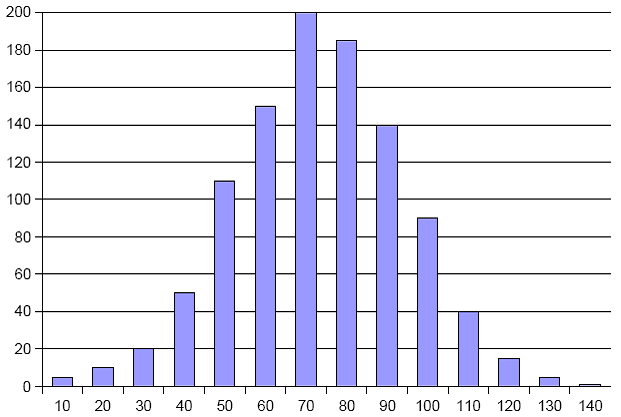
\includegraphics[width=4cm]{grafsim.png} &
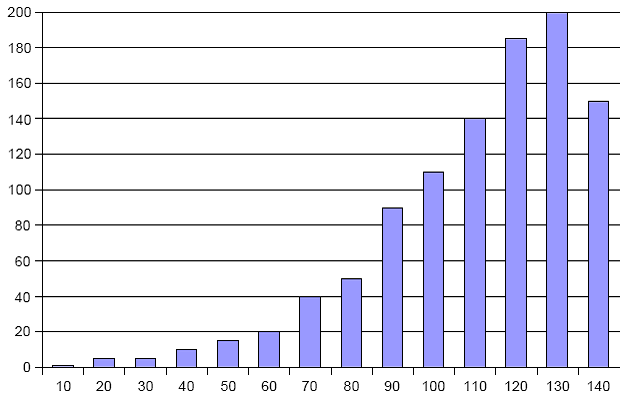
\includegraphics[width=4cm]{grafasimneg.png} &
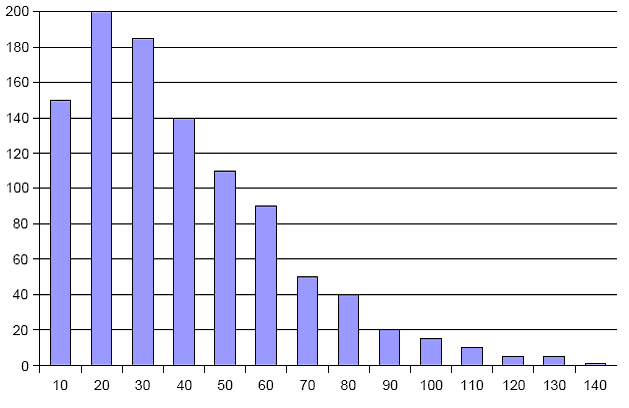
\includegraphics[width=4cm]{grafasimpos.png} \\
{\small Moda=$70$} & {\small Moda=$130$}& {\small Moda=$20$} \\
{\small Mediana=$70$} & {\small Mediana=$120$} & {\small Mediana=$30$} \\
{\small Media=$73,2$} & {\small Media=$110,78$} & {\small Media=$39,22$} 
\end{tabular}
\end{center}
\caption{Relaci\'on entre la simetr\'ia y la moda, mediana y media de una distribuci\'on 
unimodal}
\label{grafsimetria}
\end{figure}


En los tres casos el valor de la moda es \'unico (distribuciones unimodales).
Podemos observar como en la primera gr\'afica los valores de los tres estad\'isticos
son muy similares y que la gr\'afica es sim\'etrica respecto al valor central.

La segunda es asim\'etrica y se cumple que media $<$ mediana $<$ moda. Este tipo de asimetr\'ia
recibe el nombre de asimetr\'ia negativa o por la izquierda.

Finalmente, la tercera gr\'afica tambi\'en es asim\'etrica, cumpli\'endose que
moda $<$ mediana $<$ media. Esta asimetr\'ia se conoce como asimetr\'ia positiva o por la derecha.


\section{C\'alculo de moda, mediana, media y percentiles con ordenador}
\label{secCentralOrd}

Las operaciones matem\'aticas que deben realizarse para calcular los estad\'isticos
explicados en este tema son muy sencillas y pueden realizarse con una simple calculadora.
No obstante, si la cantidad de datos es elevada, programas como el OpenOffice Calc permiten 
c\'alcular f\'acilmente los estad\'isticos m\'as habituales de una distribuci\'on. 
Explicaremos c\'omo hacerlo en los si\-guien\-tes ejemplos.

\vskip 0.5 cm
\noindent
\textbf{Ejemplo 1}

Calcular la media, la moda, la mediana y los cuartiles $1^o$ y $3^o$ 
de la clasificaci\'on del RCD Mallorca durante la temporada 2005-2006 a 
partir de los datos del siguiente gr\'afico (fuente LFP): 

\begin{center}
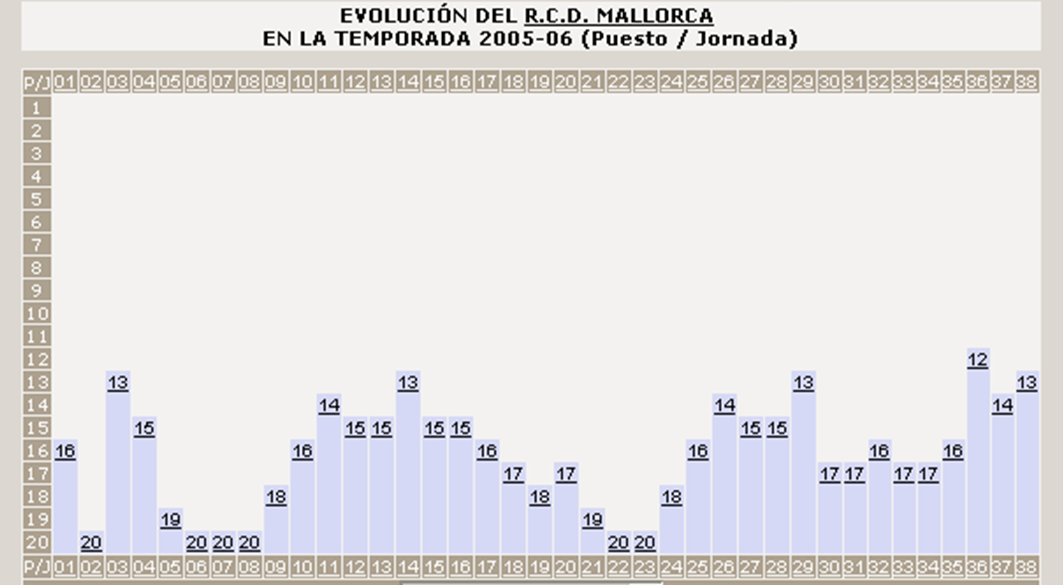
\includegraphics[width=14cm]{ejemplo5T2.png}
\end{center}

OpenOffice Calc permite calcular de forma muy sencilla la moda, mediana y media de un conjunto
de datos \textit{brutos}, es decir, no organizados en un tabla de frecuencias.
Para resolver este ejemplo seguiremos los pasos siguientes:
\begin{enumerate}
\item Al igual que en el ejemplo 5 del tema anterior, en primer lugar escribiremos los
datos \textit{brutos} en la primera columna de la hoja de c\'alculo (casillas A1 a A38).
El resultado se muestra en la figura \ref{calc1ej5}-izquierda del tema anterior.
\item A continuaci\'on escribimos las palabras ``Moda'', ``Mediana'', ``Media'', ``1er cuartil''
y ``3er cuartil'' en
las casillas $C15$, $C16$, $C17$, $C18$ y $C19$ de la hoja de c\'alculo (o en otras casillas cualesquiera)
\item \textbf{Moda}. Nos situamos en la casilla $D15$ y escribimos \verb@=Moda(A1:A38)@. Al pulsar 
\textit{Enter} obtenemos el valor de la moda.
\item \textbf{Mediana}. Nos situamos en la casilla $D16$ y escribimos \verb@=Mediana(A1:A38)@. Al pulsar 
\textit{Enter} obtenemos el valor de la mediana.
\item \textbf{Media}. Nos situamos en la casilla $D17$ y escribimos \verb@=Promedio(A1:A38)@. Al pulsar 
\textit{Enter} obtenemos el valor de la media.
\item \textbf{$1^\mathrm{er}$ cuartil}. Nos situamos en la casilla $D18$ y escribimos 
\verb@=Cuartil(A1:A38;1)@. Al pulsar \textit{Enter} obtenemos el valor del $1^\mathrm{er}$ cuartil.
\item \textbf{$3^\mathrm{er}$ cuartil}. Nos situamos en la casilla $D19$ y escribimos 
\verb@=Cuartil(A1:A38;3)@. Al pulsar \textit{Enter} obtenemos el valor del $3^\mathrm{er}$ cuartil.
\end{enumerate}

El resultado obtenido es: 
\begin{center}
\begin{tabular}{ll}
Moda & $15$ \\
Mediana & $16$ \\
Media & $16,34$ \\
$1^\mathrm{er}$ cuartil & $15$\\
$3^\mathrm{er}$ cuartil & $18$ 
\end{tabular}
\end{center}

Los tres valores centrales (moda, media y mediana) son muy similares, 
aunque se cumple que media $>$ mediana $>$ moda,
por lo que podemos afirmar que se trata de una distribuci\'on casi sim\'etrica 
con una ligera asimetr\'ia hacia la derecha.


\vskip 0.3 cm
\textbf{Nota:} al utilizar las f\'ormulas \textit{Mediana} y \textit{Cuartil} de Calc
para el c\'alculo de la mediana y el primer y tercer cuartiles los resultados obtenidos
pueden ser ligeramente diferentes a los que obtendr\'iamos con el m\'etodo que se explica 
en los ejemplos siguientes. La raz\'on es que Calc utiliza unas f\'ormulas diferentes
a las nuestras para el c\'alculo de cuartiles de datos \textit{brutos}.



\vskip 0.3 cm
\noindent
\textbf{Ejemplo 2} 

Repetir los c\'alculos del ejemplo anterior pero a partir de los
datos organizados en la tabla de frecuencias siguiente (correspondiente
al ejemplo 5 del tema 2):

\begin{center}
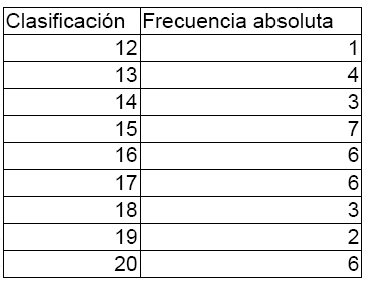
\includegraphics[width=6cm]{ejemplo1.png}
\end{center}

En este caso el c\'alculo de la media es muy sencillo pero el c\'alculo de moda y
mediana es algo m\'as complicado. A continuaci\'on explicamos c\'omo hacerlo:

\begin{enumerate}
\item En primer lugar escribimos los valores de la variable y sus frecuencias en una tabla
de OpenOffice Calc. A continuaci\'on calculamos las frecuencias y los porcentajes acumulados, tal como se
ha explicado en el tema anterior. La tabla que obtenemos es como la de la figura \ref{calc1ej1}.

\begin{figure}[htbp]
\begin{center}
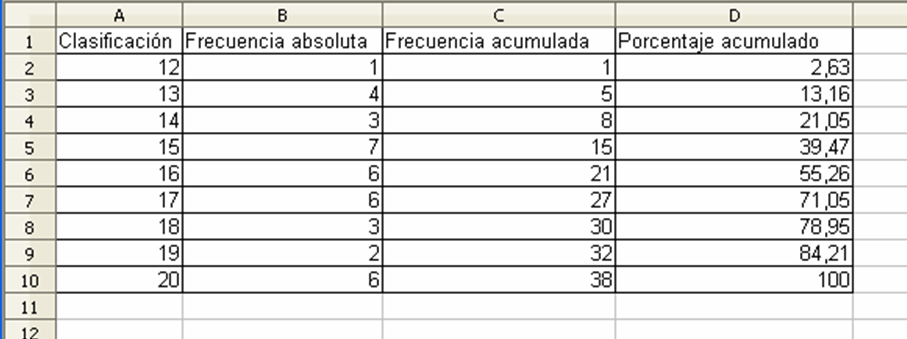
\includegraphics[width=7cm]{calc1ej1.png}
\end{center}
\caption{OpenOffice Calc con los del ejemplo 2 y las frecuencias y porcentajes acumulados calculadas}
\label{calc1ej1}
\end{figure}

\item \textbf{Moda}. En casos como el del ejemplo, en los que la tabla de datos es peque\~na
basta observar los valores de frecuencia absoluta para descubrir para qu\'e valor de la variable
tenemos un m\'aximo. En este ejemplo la moda es $15$, ya que tiene el valor de frecuencia absoluta
mayor ($7$).

Cuando la tabla de datos es muy grande, la moda se puede encontrar siguiendo el siguiente
procedimiento:
\begin{enumerate}
\item Primero copiamos los datos originales en unas nuevas columnas para evitar perderlos:
\begin{enumerate}
\item seleccionamos, manteniendo el bot\'on del rat\'on pulsado, las casillas con los valores
de la variable y sus frecuencias absolutas (en nuestro ejemplo las casillas $A2$ a $A10$ y $B2$ a $B10$),
\item pulsamos la combinaci\'on de teclas \textit{Ctrl-C} para copiar estos datos,
\item situamos el cursor en alguna otra casilla del documento (por ejemplo, $A14$), 
\item pulsamos el bot\'on derecho del rat\'on y seleccionamos la opci\'on \textit{Pegado especial...},
\item activamos la opci\'on \textit{N\'umeros} y desactivamos todas las dem\'as,
\item finalmente pulsamos \textit{Aceptar}. Los datos (s\'olo los valores num\'ericos, no las f\'ormulas)
quedan copiados en las casillas $A14$ a $A22$ y $B14$ a $B22$.
\end{enumerate}
\item Seleccionamos las casillas $A14$ a $A22$ y $B14$ a $B22$ manteniendo el bot�n izquierdo del rat\'on pulsado.
\item En el men\'u principal escogemos la opci\'on \textit{Datos}, y a continuaci\'on \textit{Ordenar...}
\item Se abre una ventana en la que se definen los criterios de ordenaci\'on. En nuestro caso
escogemos las opciones: \textit{Ordenar seg\'un:  Columna $B$} y \textit{Descendente}. Pulsamos
\textit{Aceptar}.
\item En la columna $A$ (casillas $A14$ a $A22$) aparecen los valores de la variable ordenados en orden 
decreciente de frecuencia absoluta (casillas $B14$ a $B22$), ver figura \ref{calc2ej1}.
El primer valor de la columna es la moda de la distribuci\'on. En nuestro caso: moda=$15$. 
Si la distribuci\'on fuera bimodal (el m\'aximo ocurre en dos valores de la variable), deber\'iamos
tomar como moda los dos primeros valores de la columna $A$.

\begin{figure}[htbp]
\begin{center}
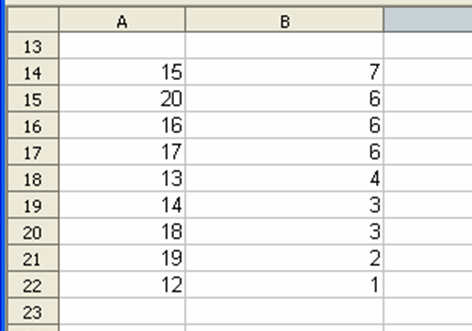
\includegraphics[width=5cm]{calc2ej1.png}
\end{center}
\caption{Ilustraci\'on del c\'alculo de la moda en el ejemplo 2}
\label{calc2ej1}
\end{figure}

\end{enumerate}
 
\item \textbf{Mediana}. La mediana es el primer valor de la columna \textit{Clasificaci�n}
cuyo porcentaje acumulado es superior o igual al $50\%$. Observando la tabla
de frecuencias de la figura \ref{calc1ej1} vemos que la mediana es $16$, ya que
su porcentaje acumulado es $55,26\%$.

\item \textbf{$1^\mathrm{er}$ cuartil}. El c\'alculo es similar al de la mediana.
El $1^\mathrm{er}$ cuartil es primer el valor de la columna \textit{Clasificaci�n}
cuyo porcentaje acumulado es superior o igual al $25\%$. Observando la tabla
de frecuencias de la figura \ref{calc1ej1} vemos que el $1^\mathrm{er}$ cuartil
es $15$, ya que su porcentaje acumulado es $39,47\%$.

\item \textbf{$3^\mathrm{er}$ cuartil}. Igual que en el caso anterior pero buscando
un porcentaje acumulado mayor o igual que $75\%$. En este caso el 
$3^\mathrm{er}$ cuartil es $18$, ya que su porcentaje acumulado es $78,95\%$.

\item \textbf{Media}. La media en este caso se calcula de manera muy 
sencilla del siguiente modo:
\begin{enumerate}
\item Situamos en cursor en una casilla vac\'ia cualquiera, por ejemplo la casilla $F2$.
\item Escribimos la f\'ormula 

\verb@=SUMA.PRODUCTO(A2:A10;B2:B10)/SUMA(B2:B10)@\footnote{Esta

f\'ormula calcula la media empleando la f\'ormula dada en la secci\'on 3.2: 
m\'ultiplica los valores de las casillas $A2$ y $B2$, $A3$ y $B3$, etc, suma
los productos y finalmente divide el total por la suma de los valores de las casillas $B2$ a $B10$}
 y 
pulsamos \textit{Enter}. El valor de la media se escribe en la casilla $F2$.
En este caso, media=$16,34$.
\end{enumerate}
 
\end{enumerate}

\vskip 0.3 cm
Por \'ultimo comentar que los valores de moda, mediana y media obtenidos son los
mismos que en el ejemplo anterior.


\vskip 0.3 cm
\noindent
\textbf{Ejemplo 3}

Calcular la mediana y la moda de la calificaci\'on de los alumnos de
\textit{Fo\-na\-ments Matem\`atics II} (Ingenier\'ia Telem\'atica) del
curso 2003-2004, a partir de los datos de la siguiente tabla (fuente UIB). 
?`Es posible calcular la media?

\begin{center}
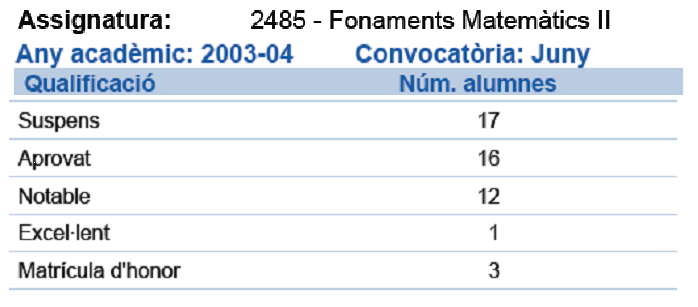
\includegraphics[width=11cm]{ejemplo2.png}
\end{center}

\vskip 0.3 cm
En este ejemplo, la variable ``Qualificaci\'o'' es una variable ordinal por lo
que no es posible calcular su media, pero s\'i $ $ su moda y mediana.

Al tratarse de una tabla con muy pocos valores la moda se encuentra f\'acilmente
observando la tabla: moda=\textit{Suspens}, ya que es el valor con la m\'axima
frecuencia absoluta.

Para calcular la mediana debemos calcular primero los porcentajes acumulados.
Lo podemos hacer en una hoja de c\'alculo de OpenOffice Calc tal como
se ha explicado en el tema anterior y obtendr\'iamos el resultado de la
figura \ref{calc1ej2}.


\begin{figure}[htbp]
\begin{center}
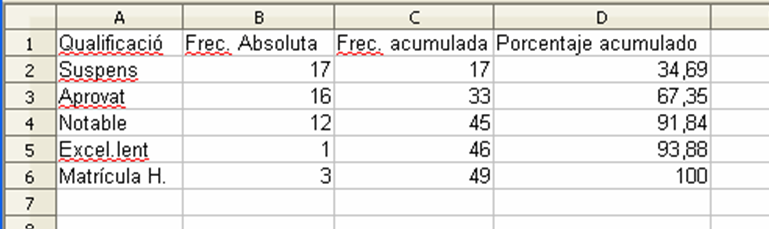
\includegraphics[width=9cm]{calc1ej2.png}
\end{center}
\caption{Izquierda: frecuencias absolutas y acumuladas para el ejemplo 3.}
\label{calc1ej2}
\end{figure}

A continuaci\'on seguimos el procedimiento explicado en el ejemplo 2 para 
el c\'alculo de la mediana: buscamos el primer valor de la columna
\textit{Qualificaci\'o} cuyo porcentaje acumulado sea superior o igual a $50\%$.
En este caso la soluci\'on es \textit{Aprovat} (porcentaje acumulado=$67,35$).

\vskip 0.2 cm
Este ejemplo muestra como el valor de la moda no explica suficientemente bien la 
distribuci\'on de valores. En este caso la moda era \textit{Suspens}, sin embargo
m\'as de la mitad de los estudiantes han aprobado (de hecho $16+12+1+3=32$ 
estudiantes aprueban, exactamente el doble de alumnos suspendidos). 
La mediana describe de manera mejor los valores de la variable al dar un valor de 
\textit{Aprovat}.

\vskip 0.3 cm
\noindent
\textbf{Ejemplo 4}

Calcular la moda y la mediana de la edad de los condenados
en Illes Balears en 2005 a partir de los datos de la siguiente
tabla. Calcular los cuartiles primero y tercero.
?`Es posible calcular la media?
Si la respuesta es negativa, ?`como estimar\'ias de manera
aproximada el valor de la media?

\begin{center}
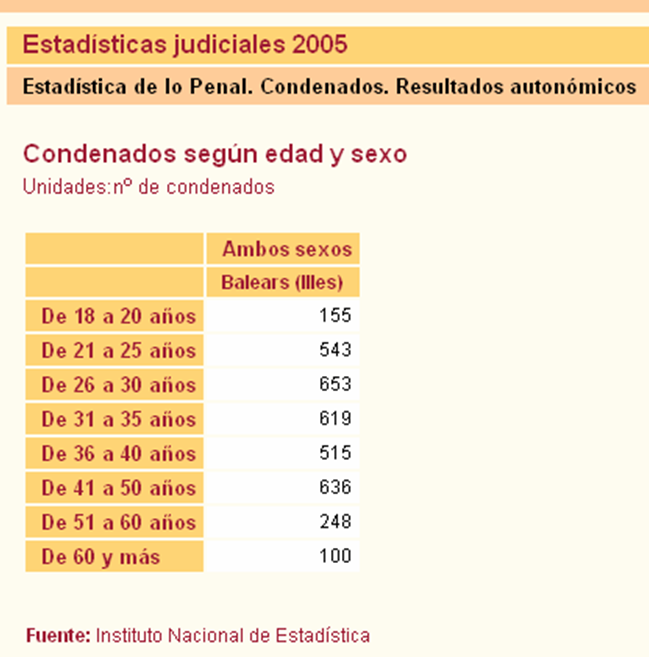
\includegraphics[width=11cm, height=7cm]{ejemplo3.png}
\end{center}

\vskip 0.2 cm
Se trata de datos agrupados en forma de intervalos, de manera que calcularemos los estad\'isticos
siguiendo el procedimiento explicado en la secci\'on \ref{secintervals}:

\begin{enumerate}
\item \textbf{Moda}. Observando la tabla vemos que el valor m\'aximo se da en el intervalo
$26-30$. La moda se calcula como el valor medio del intervalo, es decir: moda=$\frac{26+30}{2}=28$.

\item \textbf{Mediana}. Calculamos las frecuencias acumuladas para cada intervalo y seguimos el
procedimiento descrito en el ejemplo 2 para hallar la mediana. En este caso, la mediana
se encuentra en el intervalo $31-35$ (ver figura \ref{calc1ej3}).

\begin{figure}[htbp]
\begin{center}
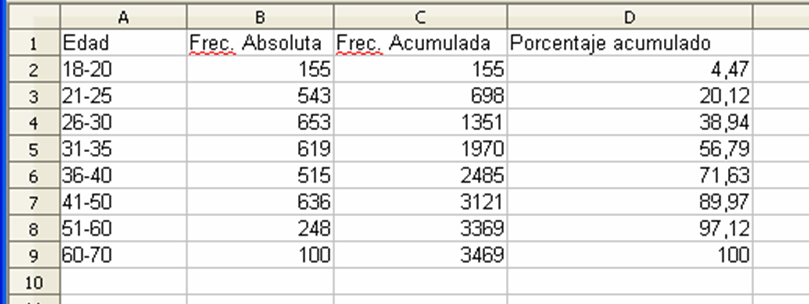
\includegraphics[width=11cm]{calc1ej3.png}
\end{center}
\caption{Tabla de frecuencias absolutas y acumuladas y porcentajes acumulados para el ejemplo 3.}
\label{calc1ej3}
\end{figure}

Para calcular de modo m\'as preciso la mediana utilizamos la f\'ormula de la secci\'on \ref{secintervals}:

\[
\mathrm{mediana}=L_i + \frac{ 50\% \cdot N - N_{i-1} }{n_{i}} \cdot (L_{i+1}-L_i)
\]
\noindent
donde $L_i$ y $L_{i+1}$ denotan los l\'imites inferior y superior del intervalo,
$n_{i}$ es la frecuencia del intervalo, $N_{i-1}$ es la frecuencia acumulada
en el intervalo anterior y $N$ es la suma de todas las frecuencias

En nuestro caso: $L_i=31$, $L_{i+1}=35$, $n_{i}=619$, $N_{i-1}=1351$ y $N=3469$,
por tanto
\[
\begin{array}{ll}
\mathrm{mediana}&=31+\frac{ 50\% \cdot 3469 - 1351 }{619} \cdot (35-31) = \\ \\
&= 31 + \frac{1734,5-1351}{619} \cdot 4 = 33,48
\end{array}
\]

\vskip 0.3 cm
El c\'alculo de los cuartiles es muy similar al de la mediana. Primero hallamos los intervalos
en los que se encuentra cada uno de ellos, si\-guien\-do un procedimiento similar
al explicado en el ejemplo 2. A continuaci\'on aplicamos
la f\'ormula explicada en la secci\'on \ref{secintervals}:

\begin{itemize}
\item \textbf{Primer cuartil}.
$L_i=26$, $L_{i+1}=30$, $n_{i}=653$, $N_{i-1}=698$ y $N=3469$
\[
26+\frac{ 25\% \cdot 3469 - 698 }{653} \cdot (30-26) = 
26 + \frac{867.25-698}{653} \cdot 4 = 27,04
\]

\item \textbf{Tercer cuartil}. 
$L_i=41$, $L_{i+1}=50$, $n_{i}=636$, $N_{i-1}=2485$ y $N=3469$
\[
41+\frac{ 75\% \cdot 3469 - 2485 }{636} \cdot (50-41) = 
41 + \frac{2601.75-2485}{636} \cdot 9 = 42,65
\]

\end{itemize}

\item \textbf{Media}. Para calcular la media de unos valores agrupados en intervalos
el primer paso consiste en calcular el valor medio de cada intervalo. En este ejemplo
sin embargo tenemos el problema de que para el �ltimo intervalo no podemos calcular
el valor medio, ya que est� definido como \textit{60 y m\'as} y no conocemos el l\'imite
superior:

En estos casos podemos calcular la media de manera aproximada haciendo alguna suposici\'on
razonable sobre el valor m\'aximo del intervalo desconocido.
A continuaci\'on explicamos el procedimiento a seguir si suponemos que el valor m\'aximo
del intervalo es $70$:

\begin{enumerate}
\item Partimos de un documento OpenOffice Calc en el que hemos creado una tabla
de frecuencias absolutas y acumuladas como la que se muestra en la figura \ref{calc1ej3}.
\item Insertamos una nueva columna a la derecha de la columna $A$. Para ello situamos
el cursor sobre la parte superior de la columna $B$, hacemos clic en el bot\'on
derecho del rat\'on y elegimos la opci\'on \textit{insertar columnas}.
Una nueva columna $B$ aparece y las columnas $B$, $C$, $D$, etc
se desplazan hacia a la derecha (ver figura \ref{calc2ej3}-arriba).
\item En la primera casilla de la nueva columna escribimos \textit{Edad media}
y en las casillas inferiores escribimos las f\'ormulas que calculan los valores medios de los
intervalos: \verb@=(18+20)/2@, \textit{Enter} (casilla $B2$);
\verb@=(21+25)/2@, \textit{Enter} (casilla $B3$); etc. Finalmente, para la casilla
$B9$ \textit{suponemos} que el valor m\'aximo del intervalo es $70$ y escribimos \verb@=(60+70)/2@.
La tabla resultante tiene la forma que se muestra en la figura \ref{calc2ej3}-abajo.


\begin{figure}[htbp]
\begin{center}
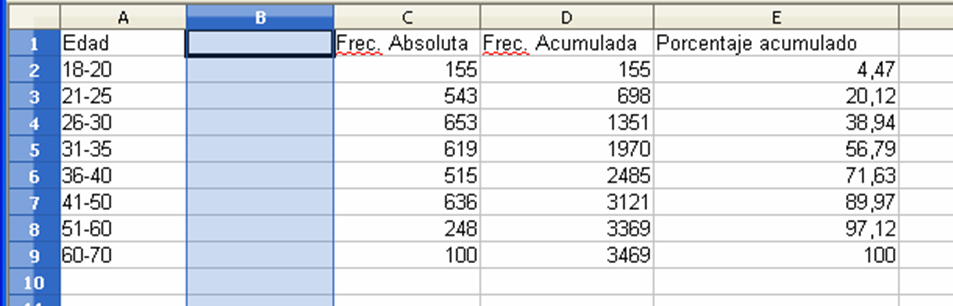
\includegraphics[width=8cm]{calc2ej3.png}
\vskip 0.3 cm
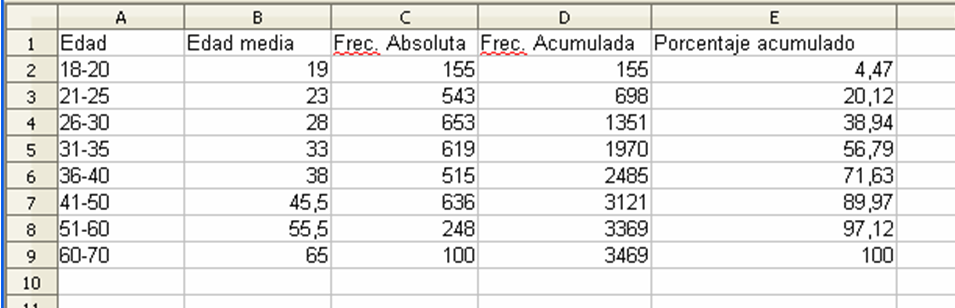
\includegraphics[width=8cm]{calc3ej3.png}
\end{center}
\caption{Tablas de frecuencias y porcentajes para el ejemplo 3. Arriba, inserci�n de una
nueva columna. Abajo, datos insertados con los valores centrales
de los intervalos}
\label{calc2ej3}
\end{figure}

\item El calculo de la media se hace ahora de manera similar al ejemplo 2:

\begin{enumerate}
\item Situamos en cursor en una casilla vac\'ia cualquiera, por ejemplo la casilla $A12$.
\item Escribimos la f\'ormula 

\verb@=SUMA.PRODUCTO(B2:B9;C2:C9)/SUMA(C2:C9)@ y 

pulsamos \textit{Enter}. El valor de la media se escribe en la casilla $A12$.
En este caso, media=$35,43$.
\end{enumerate}

\end{enumerate}


Como comentario final decir que otras suposiciones razonables sobre el 
valor m\'aximo del intervalo \textit{$60$ y m\'as} hubieran producido
resultados similares. Por ejemplo, para la suposici\'on $60-65$
hubi\'eramos obtenido media=$35,36$; 
para $60-75$, media=$35,51$;
para $60-80$, media=$35,58$, etc.
Lo importante es no suponer valores absurdos (por ejemplo $60-150$,
pues es muy poco probable que haya personas de 150 a\~nos que cometan delitos).


\end{enumerate}



\vskip 0.3 cm
\noindent
\textbf{Ejemplo 5}

Calcular los estad\'isticos de tendencia central asociados a la variable ``tipo de
infracci\'on'' a partir de los datos de la siguiente tabla:

\begin{center}
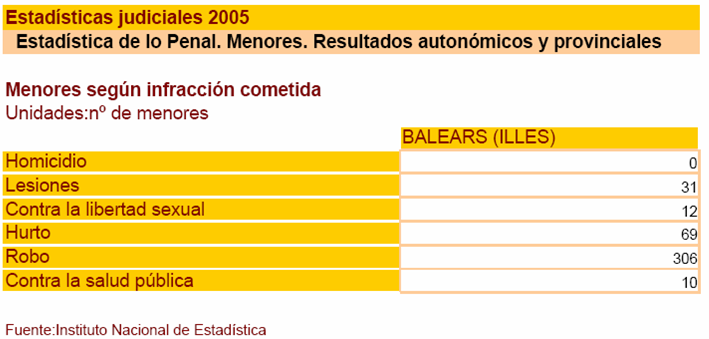
\includegraphics[width=12cm]{ejemplo4.png}
\end{center}

Se trata de una variable cualitativa por lo que el \'unico estad\'istico que podemos
calcular es la moda. Observando la tabla vemos que el valor m\'aximo de frecuencia es $306$,
que corresponde al valor \textit{Robo}. Por lo que concluimos que: moda=\textit{Robo}.

\vskip 0.3 cm
\noindent
\textbf{Ejemplo 6}

Calcular los estad\'isticos de tendencia central asociados a la variable 
``autobuses matriculados por mes durante el a\~no 2006'' 
a partir de los datos de la siguiente tabla (fuente DGT):

\begin{center}
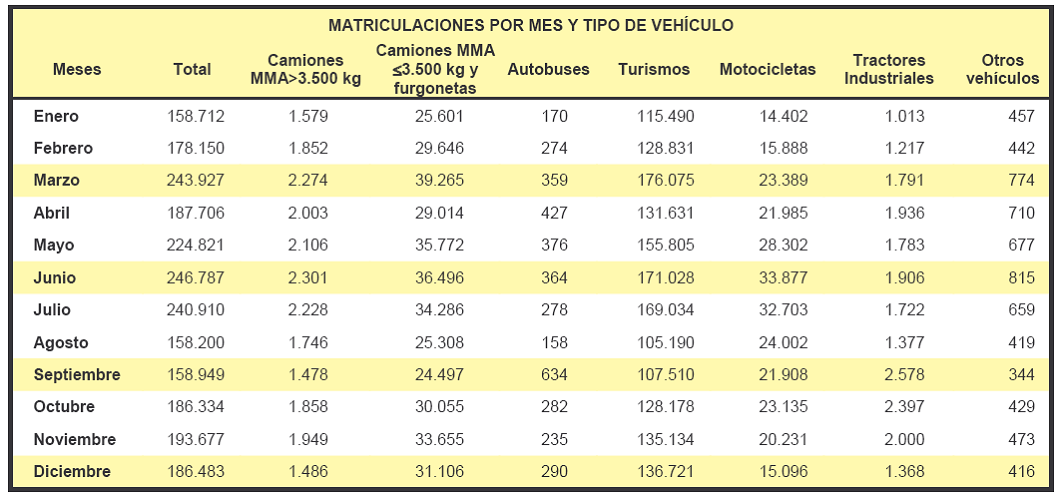
\includegraphics[width=14cm]{ejemplo5.png}
\end{center}

Los datos de la tabla son valores \textit{en bruto}, por lo que aplicamos el procedimiento
explicado en el ejemplo 1:

\begin{enumerate}
\item Escribimos los datos \textit{brutos} en la primera columna de la hoja de c\'alculo 
(ca\-si\-llas $A1$ a $A12$).
El resultado se muestra en la figura \ref{calc1ej5T2}.

\begin{figure}[htbp]
\begin{center}
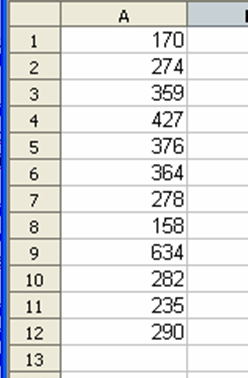
\includegraphics[width=3cm]{calc1ej5T2.png}
\end{center}
\caption{Datos brutos del ejemplo 6}
\label{calc1ej5T2}
\end{figure}

\item A continuaci\'on escribimos las palabras ``Moda'', ``Media'', ``Mediana'', ``1er cuartil''
y ``3er cuartil'' en
las casillas $C15$, $C16$, $C17$, $C18$ y $C19$ de la hoja de c\'alculo (o en otras casillas cualesquiera)
\item \textbf{Moda}. Nos situamos en la casilla $D15$ y escribimos \verb@=Moda(A1:A12)@. Al pulsar 
\textit{Enter} obtenemos el valor de la moda. En este caso obtenemos un mensaje de error
pues todos los valores ocurren una \'unica vez. Esto significa que el c\'alculo de la moda
no tiene sentido en este problema.
\item \textbf{Media}. Nos situamos en la casilla $D16$ y escribimos \verb@=Promedio(A1:A12)@. Al pulsar 
\textit{Enter} obtenemos el valor de la media.
\item \textbf{Mediana}. Nos situamos en la casilla $D17$ y escribimos \verb@=Mediana(A1:A12)@. Al pulsar 
\textit{Enter} obtenemos el valor de la mediana.
\item \textbf{$1^{er}$ cuartil}. Nos situamos en la casilla $D18$ y escribimos \verb@=Cuartil(A1:A12;1)@. 
Al pulsar \textit{Enter} obtenemos el valor del primer cuartil.
\item \textbf{$3^{er}$ cuartil}. Nos situamos en la casilla $D19$ y escribimos \verb@=Cuartil(A1:A12;3)@. 
Al pulsar \textit{Enter} obtenemos el valor del tercer cuartil.
\end{enumerate}

El resultado obtenido es: 
\begin{center}
\begin{tabular}{ll}
Media & $320,58$ \\
Mediana & $286$ \\
$1^{er}$ cuartil & $264,25$ \\
$3^{er}$ cuartil & $367$ \\
\end{tabular}
\end{center}

\vskip 0.3 cm
\textbf{Nota:} si para el c\'alculo de la mediana y cuartiles hubi\'eramos calculado
primero la tabla de frecuencias absolutas de cada valor y a continuaci\'on hub\'eramos 
hecho el c\'alculo con el procedimiento explicado en los ejemplos anteriores, los resultados
hubieran sido ligeramente diferentes: mediana=$282$, $1^{er}$ cuartil=$235$ y 
$3^{er}$ cuartil=$364$. La raz\'on es que Calc utiliza unas f\'ormulas diferentes
a las nuestras para el c\'alculo de cuartiles para datos \textit{brutos}.

\section{Ejercicios propuestos}


\vskip 0.2 cm
\noindent
\textbf{Ejercicio 1} 

A partir de los datos de la siguiente tabla calcular los estad\'isticos de tendencia 
central para la variable ``Edad de v\'ictimas de accidentes en 2006''. Calcular tambi\'en
el primer y el tercer cuartiles.
\vskip 0.2 cm
\begin{center}
\begin{tabular}{c|c}
Edad (a\~nos) & $N^o$ v\'ictimas \\ \hline
0 a 4 & 343 \\ 
5 a 14 & 1172 \\
15 a 17 & 333 \\
18 a 24 & 918 \\
25 a 64 & 5026 \\
65 y m\'as & 2947
\end{tabular}

Edad de v\'ictimas de accidentes en 2006 (fuente DGT)
\end{center}


\vskip 0.5 cm
\noindent
\textbf{Ejercicio 2} 

Calcular los estad\'isticos de tendencia central y los cuartiles $1^o$ y $3^o$
asociados a la variable ``turismos matriculados por mes durante el a\~no 2006'' 
a partir de los datos de la tabla del ejemplo 6.



\vskip 0.5 cm
\noindent
\textbf{Ejercicio 3} 

Calcular los estad\'isticos de tendencia central asociados a la variable ``tipo de
alojamiento'' a partir de los datos de la siguiente tabla (fuente INE):

\begin{center}
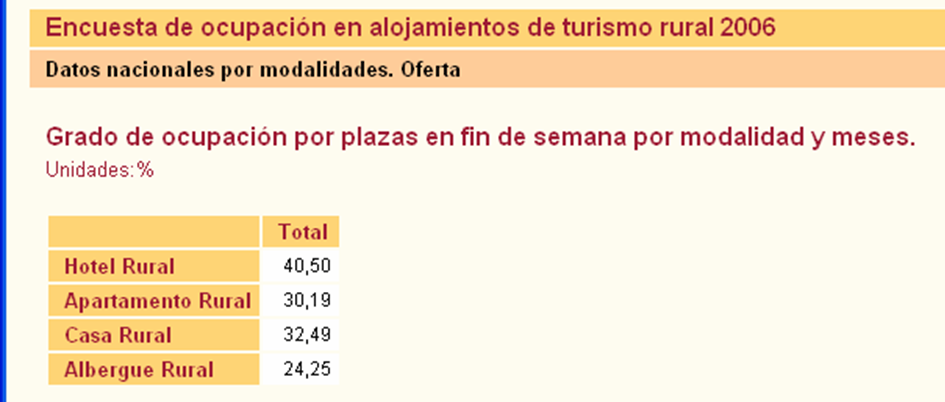
\includegraphics[width=12cm]{ejercicio3.png}
\end{center}

\vskip 0.5 cm
\noindent
\textbf{Ejercicio 4} 

Calcular los estad\'isticos de tendencia central y los cuartiles $1^o$ y $3^o$
de la variable
``terminaci\'on del cup\'on de la ONCE en el per\'iodo 30 de octubre a 27 de noviembre de 2007''
a partir de los datos de la siguiente tabla (fuente ONCE). 
?`Qu\'e tipo de simetr\'ia presenta la distribuci\'on? 

\vskip 0.2 cm
\begin{center}
\begin{tabular}{c|c}
Terminaci\'on & Frecuencia \\ \hline
0 & 0 \\
1 & 4 \\
2 &  0\\
3 &  2\\
4 &  2\\
5 &  3\\
6 &  3\\
7 &  6\\
8 &  3\\
9 &  1 
\end{tabular}
\end{center}



\vskip 0.5 cm
\noindent
\textbf{Ejercicio 5}

Calcular los estad\'isticos de tendencia central del grado de satisfaci\'on
de los clientes de un determinado establecimiento a partir de los datos siguientes:
\vskip 0.2 cm
\begin{center} 
\begin{tabular}{c|c}
Grado satisfacci\'on & $N^o$ clientes \\ \hline
Muy satisfecho & 50 \\
Bastante satisfecho & 80 \\
Satisfecho & 100 \\
Poco satisfecho & 40 \\
Nada satisfecho & 10
\end{tabular}
\end{center}

%\section{Soluciones de los ejercicios}









